\documentclass[12pt,titlepage,oneside]{article}
\usepackage{titlesec}
\titlelabel{\thetitle. }
\setlength{\footskip}{100pt}
\usepackage[italian]{babel}
\usepackage[utf8]{inputenc}
\usepackage{listings} 
\usepackage{comment} 
\usepackage{cite}\usepackage{}
\usepackage{float}
\usepackage[table,xcdraw]{xcolor}
\lstset{
    literate={~} {$\sim$}{1}
}
\usepackage{amsmath,amssymb,amsfonts,amsthm,graphicx,mathrsfs,braket}
\usepackage{hyperref}
\usepackage{times}
\usepackage[left=2.5cm, right=2.5cm]{geometry}
\usepackage{xcolor}
\usepackage{algorithm}
\usepackage[noend]{algpseudocode}
\makeatletter
\def\BState{\State\hskip-\ALG@thistlm}
\makeatother
\hypersetup{colorlinks=false,
allbordercolors=white}
\setcounter{secnumdepth}{4} 
\setcounter{tocdepth}{3}
\linespread{1.5}
\usepackage[a-1b]{pdfx}
\usepackage{xcolor}
\definecolor{stringcolor}{rgb}{0,0.568,0.541}
\definecolor{codegray}{rgb}{0.5,0.5,0.5}
\definecolor{darkblue}{HTML}{152c6b}
\definecolor{codegreen}{HTML}{799662}
\definecolor{orange}{HTML}{c28e00}
\definecolor{backcolour}{HTML}{f9f9f9}
\definecolor{linecolor}{rgb}{0.1, 0.1, 0.1}
\usepackage[skip=1cm]{caption}
\usepackage{subcaption}
\usepackage[export]{adjustbox}

\begin{document}

\newcommand\tab[1][1cm]{\hspace*{#1}}
\thispagestyle{empty}
\begin{titlepage}
\centering

\begin{figure*}[!t]
	\begin{center}
		
\includegraphics[width=0.25\columnwidth]{logo.png}
	\end{center}
\end{figure*}

{\Large \textbf{UNIVERSIT\`A DEGLI STUDI DI CATANIA}}

{\scshape
\large
Dipartimento di Matematica e Informatica
}

{\scshape
\normalsize
Corso di Laurea Magistrale in Informatica
}

\bigskip


\hrule

\vspace{1cm}

{\itshape
\large
Valerio Tosto
\par}

\vspace{0.5cm}


{\centering
\Large
RISOLUZIONE DEL GRAPH PARTITIONING PROBLEM MEDIANTE L'APPLICAZIONE DELL'ITERATED LOCAL SEARCH
\par}

\vspace{1.5cm}


\begin{minipage}[b]{8 cm}
\hrule

\bigskip

{\centering\scshape 
Relazione progetto Intelligenza Artificiale
\par}


\bigskip

\hrule
\end{minipage}

\vspace{2.4cm}


\hrule

\bigskip


{\centering
Anno Accademico 2020 - 2021
\par}
\end{titlepage}

\clearpage
\tableofcontents

\clearpage
\section{Descrizione del problema}
\textit{Il graph partitioning problem consiste nel trovare un partizionamento di un grafo $G = (V, E)$ in $K$ sottoinsiemi di vertici $V_1, V_2, \ldots, V_K$ con $|V_1| = |V_2| = \ldots = |V_K|$ in modo tale che il numero di archi che collegano i vertici di differenti partizioni sia ridotto al minimo.\\
Il problema assegnato fissa $K=2$ e rimuove il vincolo del bilanciamento perfetto (ammesso uno sbilanciamento massimo del $5\%$), pur mantenendo l'obiettivo di individuare il cut-size minimo sul grafo bi-partizionato}

\section{Istanze}
\textit{Le istanze del problema sono state fornite mediante file .graph; esso è composto da una prima riga contenente le cardinalità di vertici ed archi e da successive righe ove ogni riga i-esima indica la sequenza dei nodi adiacenti al nodo i.
Il progetto è stato sviluppato e continuamente affinato su due istanze di grafo di test:}
\begin{itemize}
  \item test.graph
  \item test.100.graph
\end{itemize}
\textit{Entrambe le istanze sono state create a partire dall'add20.graph e contengono rispettivamente 16 e 99 nodi. L'uso di esse, seppur a prima vista poco funzionale, ha permesso di affinare le logiche implementate e di verificarne la bontà mediante il plotting della soluzione iniziale e finale.\\
Infine, per verificare le performance dell'algoritmo, è stato fatto uso delle 3 istanze fornite:}
\begin{itemize}
  \item 3elt.graph
  \item add32.graph
  \item add20.graph
\end{itemize}

\section{Algoritmo di risoluzione}
\textit{Tra gli algoritmi di risoluzione proposti, è stato scelto di adottare l'Iterated Local Search. Esso fornisce notevoli vantaggi in quanto, partendo da una soluzione iniziale $S_0$, permette di individuare un ottimo locale e, mediante perturbazioni, spostarsi dall'intervallo di soluzioni trovato nel tentativo di scovare un eventuale ottimo globale; si ritiene che il fattore di casualità presente nell'Iterated Local Search possa offrire un boost nella ricerca dell'ottimo globale se confrontato con gli altri algoritmi proposti.}

%\clearpage
\section{Iterated Local Search}
\textit{L'algoritmo di Iterated Local Search prevede la generazione di una soluzione iniziale $S_0$, sulla quale eseguire l'algoritmo di Local Search e, fino al raggiungimento di uno stop criteria:}
\begin{itemize}
  \item una perturbazione $S'$ della soluzione $S^*$ precedentemente ottenuta
  \item una Local Search a partire da $S'$ 
  \item l'accettazione tra la soluzione $S'$ e la $S'^*$ precedentemente ottenuta
\end{itemize}
\textit{La scelta della soluzione da eccettare può giocare un ruolo chiave, congiuntamente alla perturbazione della Local Search, per spostarsi dal punto di ottimo locale, in cerca di un possibile ottimo globale.\\
La prima implementazione effettuata prevedeva, pertanto, l'accettazione di una soluzione "peggiorativa" fino ad un massimo del $5\%$ della funzione obiettivo, ma è stata successivamente scartata in quanto "penalizzante" su un basso numero di iterazioni all'interno della Local Search.}

\section{Generazione della soluzione iniziale}
\textit{Seppur non strettamente necessario, si è voluto ugualmente sviluppare l'algoritmo in maniera tale da fornire sempre un grafo bilanciato. Ci si è dunque orientati a selezionare randomicamente i $|V|/2$ nodi da assegnare alla Partizione 1; quelli non selezionati sono stati pertanto assegnati alla Partizione 0.\\
La scelta di adottare una soluzione randomica piuttosto che un algoritmo greedy ha il vantaggio di testare le performance dell'algoritmo indipendentemente dalla soluzione iniziale e di differenziarla maggiormente per ogni specifica run.}

\section{Local Search}
\textit{Il classico algoritmo di Local Search, presa in input una soluzione $S_0$, prevede la generazione delle soluzioni candidate e la selezione della migliore soluzione $S_t$ fino al raggiungimento di uno stop criteria.\\
Al fine di migliorare il risultato ottenuto, si è optato per l'aggiunta di un nuovo step, eseguito ad ogni iterazione interna alla Local Searh: lo switch dei nodi isolati. Per nodo isolato si intende quel nodo avente il massimo rapporto tra nodi esterni alla partizione e nodi raggiungibili da esso.\\
Inizialmente implementato per riassegnare un singolo nodo isolato per partizione, è stato successivamente rivisto per selezionare e riassegnare un numero eguale di nodi isolati. Ogni esecuzione dello "switch isolated nodes" fornisce in output una nuova soluzione $S_ts$; essa verrà considerata come nuova soluzione di partenza, per la successiva generazione di soluzioni candidate, solo nel caso in cui la funzione obiettivo (min cut-size) venga migliorata.}

\clearpage
\section{Generazione dei candidati}
\textit{Sono state eseguite varie prove in merito a questo fondamentale punto:}
\begin{itemize}
  \item ricerca di tutte le possibili soluzioni
  \item individuazione del nodo "più promettente" sull'intero grafo e generazione delle soluzioni ad esso vicine
  \item individuazione del nodo "più promettente" sulla singola partizione e generazione delle soluzioni ad esso vicine
\end{itemize}
\textit{La scelta finale è ricaduta su quella che fornisce il miglior compromesso tra risultato e tempo di elaborazione. Si è quindi scelto di non generare ad ogni step tutte le possibili soluzioni bensì di selezionare, per entrambe le partizioni, il nodo avente il maggior numero di vicini esterni alla partizione ed il minor numero di vicini interni alla partizione.\\
Effettuata questa scelta, si è provveduto alla generazione di tutte le soluzioni possibili mediante lo swap del nodo individuato con ciascuno dei nodi vicini.\\
Dalle prove effettuate su test.graph, test.100.graph e add20.graph, il risparmio temporale è tale da supportare tale scelta.}

\section{Selezione dei candidati}
\textit{Presa in input una lista di soluzioni candidate, viene restituita quella che migliora maggiormente la funzione obiettivo. La scelta effettuata, seppur banale (si sarebbe potuto optare per un criterio differente), è stata ponderata in considerazione del fatto che un eventuale "peggioramento" della soluzione è concesso all'algoritmo mediante la perturbazione presente nell'Iterated Local Search; si conviene pertanto che la scelta più accurata sia quella che permetta di raggiungere più velocemente il punto di minimo locale.}

\clearpage
\section{Risultati}
\textit{In merito a questo fondamentale punto, sono state eseguite varie prove.
Si è inizialmente adottata la ricerca della miglior soluzione possibile all'interno della local search; pur portando notevoli risultati dal punto di vista del risultato ottenuto, fornendo in input un grafo di dimensioni notevolmente più elevato rispetto a quello di test, il tempo necessario all'algoritmo non è stato ritenuto accettabile.\\
Sono quindi state sondate altre strade: ricerca con arresto fisso (50 o 100 iterazioni) all'interno della local search e misto (ricerca della miglior soluzione entro un numero di iterazioni proporzionato al numero di archi/nodi del grafo); quest'ultima ha fornito un buon compromesso tra il cut-size calcolato e tempo di elaborazione.\\
Di seguito sono elencate le performance ottenute sulle istanze a disposizione con un numero di iterazioni pari al $5\%$ del numero di archi presenti nel grafo:}
\begin{table}[ht!]
\begin{tabular}{ |p{3.5cm}||p{3.5cm}|p{3.5cm}|p{3.5cm}|  }
 \hline
 \multicolumn{4}{|c|}{Performance}\\
 \hline
  & best solution & mean solutions & standard deviation\\
 \hline
 3elt.graph & N.A. & N.A. & N.A.\\
 add32.graph & N.A. & N.A. & N.A.\\
 add20.graph & N.A. & N.A. & N.A.\\
 test.100.graph & 16 & 16 & 0.0\\
 test.graph & 5 & 5 & 0.0\\
 \hline
\end{tabular}
\end{table}

\textit{Come è possibile notare dalla tabella precedente e dalle immagini sottostanti, l'ILS fornisce ottimi risultati se correttamente configurato.}
\begin{figure}
  \begin{center}
    \begin{subfigure}[b]{0.5\textwidth}
        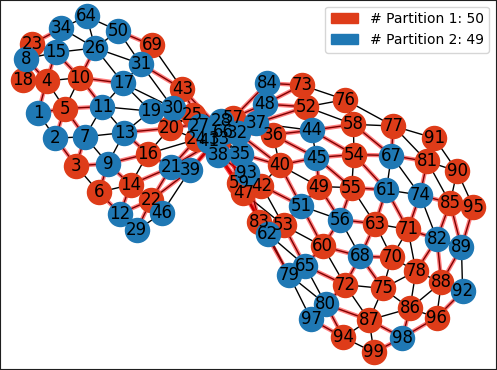
\includegraphics[scale=0.65, center]{Test100_Original_Partitions.png}
        \caption{Soluzione iniziale}
        \label{fig:test100_original}
    \end{subfigure}
    \begin{subfigure}[b]{0.5\textwidth}
        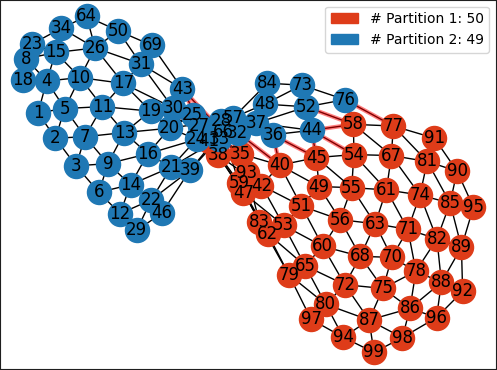
\includegraphics[scale=0.65, center]{Test100_Final_ILS_Partitions.png}
        \caption{Soluzione finale}
        \label{fig:test100_final}
    \end{subfigure}
      \caption{Esempio di soluzione iniziale e finale su test.100.graph, con numero di iterazioni pari al $5\%$ del numero di archi presenti nel grafo}
      \label{fig:three graphs}
  \end{center}
\end{figure}

\clearpage
\textit{A causa dell'esiguo tempo a disposizione, non è stato possibile affinare i risultati con un numero di iterazioni pari al $5\%$ del numero di archi; si è quindi deciso di ridurre le iterazioni allo $0.5\%$ del numero di nodi presenti nel grafo:}
\begin{table}[h!]
\begin{tabular}{ |p{3.5cm}||p{3.5cm}|p{3.5cm}|p{3.5cm}|  }
 \hline
 \multicolumn{4}{|c|}{Performance}\\
 \hline
  & best solution & mean solutions & standard deviation\\
 \hline
 3elt.graph & 1385 & 1557 & 88.00378779726852\\
 add32.graph & 1876 & 1910.2 & 22.409323456494125\\
 add20.graph & 1470 & 1554 & 71.42984125855399\\
 test.100.graph & 93 & 97.9 & 3.5103022978402048\\
 test.graph & 11 & 12.7 & 1.636391694484477\\
 \hline
\end{tabular}
\end{table}

\textit{In conclusione, il numero di iterazioni dell'algoritmo di Local Search è un fattore determinante per il raggiungimento di un miglior risultato; ciò nonostante non lede la bontà dell'algoritmo di Iterated Local Search sviluppato.}

\end{document}